%\begin{figure}[ht]
%    \centering
%    \sbox0{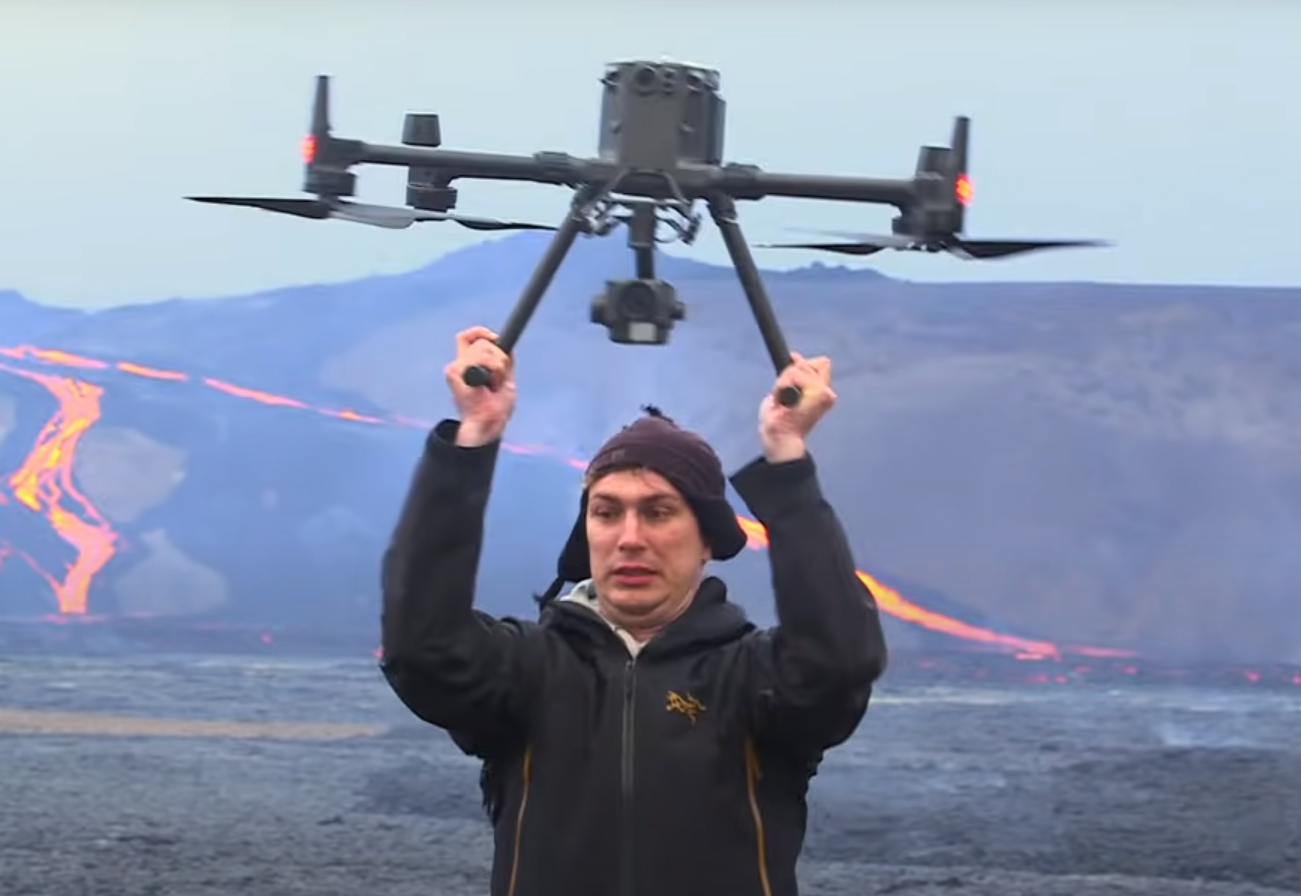
\includegraphics[width=10cm]{human_assisted_landing}}
%    \begin{minipage}{\wd0}
%      \usebox0
%      \caption{Non-ideal, human-assisted landing of Christopher Hamilton's Matrice 300 at the Fagradalsfjall volcano in the absence of a safe, autonomous landing method that considers the surrounding environment.}
%      \label{figure:hand_landing}
%    \end{minipage}
%\end{figure}

\begin{figure}[ht]
    \centering
    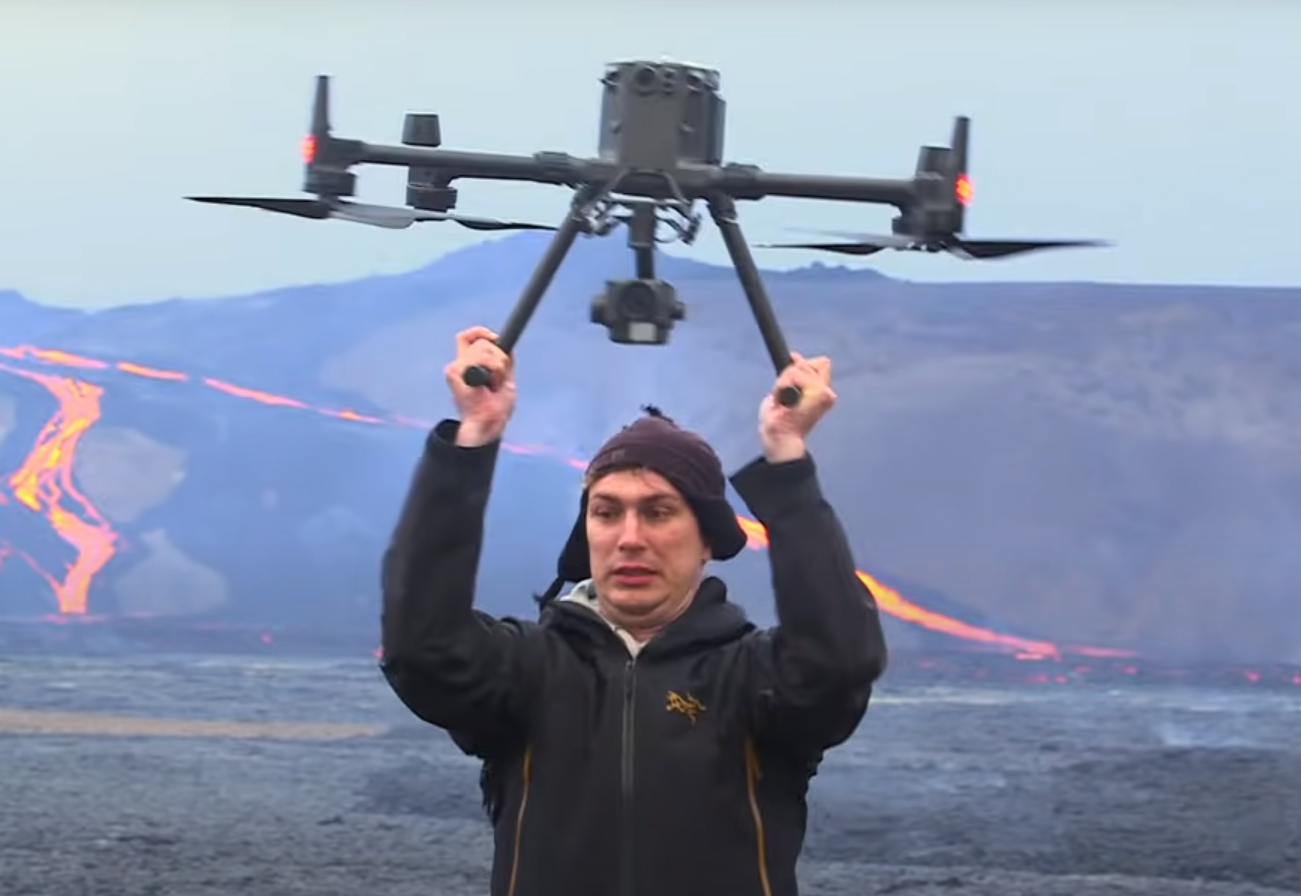
\includegraphics[width=10cm]{human_assisted_landing}
      \caption{Non-ideal, human-assisted landing of Christopher Hamilton's Matrice 300 at the Fagradalsfjall volcano in the absence of a safe, autonomous landing method that considers the surrounding environment.}
      \label{figure:hand_landing}
\end{figure}

\section{Problem Statement and Motivation}

The goal of the proposed research is to explore the topic of
autonomous, unstructured drone landing.
Current autonomous landing methods have at least one of the following disadvantages:
they are blind to obstacles,
they require \textit{known} landing sites,
or they depend on sophisticated ground control stations for offloading of expensive computation.
The proposed research targets a gap in current autonomous landing methods.
Specifically, we aim to develop a method for quickly analyzing terrain
and identifying safe landing sites using only embedded computational hardware
and a minimal set of sensors (and then carry out the landing).

Landing is a particularly difficult aspect of drone flight,
owing mainly to its risky nature and required precision.
As a result, most drone landings are carried out by a human operator,
inherently limiting the applicability of autonomous drones.
Some autopilot software includes an API for \textit{precision landing},
which allows a drone to localize and direct itself with respect to a landing pad during an autonomous landing,
according to data provided by external sensors and programs.
However, there is no particular method of autonomous landing in widespread use.
As autonomous and semi-autonomous drones are not able to reliably handle landings
on rough terrain or in non-ideal conditions, human operators often disable
autonomous control during landing (opting for full manual control),
or abuse/hack the landing system by descending to a low altitude,
grabbing hold of the drone,
and disabling the motors,
as shown in Figure~\ref{figure:hand_landing}.
Aside from potentially exposing users to dangerous rotors,
this landing technique showcases the limitations induced by a lack of
autonomous landing method.

In sufficiently flat, large areas, fully autonomous drone missions can end with a GPS-based
autonomous landing which is blind to obstacles in the environment.
However,
intuitively and demonstrably,
this can lead to crash-landings at landing sites that have obstacles within
the error radius of the GPS,
which can be anywhere from a few centimeters to a few meters.
In the available open source autopilot softwares,
obstacles are simply not handled,
and drones will continue their landing attempts even if fatally obstructed.
A proven alternative to depending on GPS for landing is to provide additional infrastructure at the landing area
to help the drone navigate reliably, e.g.~IR beacons, fiducial markers, or even ground-based cameras that identify and direct the drone.
However, this paradigm requires additional overhead, in that the landing site should be sophisticated and known ahead of time.

Some methods for autonomous landing employ in-depth topological analysis of the environment,
which are computationally- and power-intensive.
Due to the hardware onboard most drones, which is limited in terms of power and computational performance,
it is often necessary to stream data from the drone to a more powerful ground station to carry out this analysis.
However, this adds the requirement of a two-way data link between the drone and the ground station,
which limits the range of the drone, adds potentially prohibitive latency, and increases operational overhead.

Therefore, the goal of this research is to determine which methods a drone can use for autonomous landing in unknown environments,
to determine the data those methods require, and to determine how those methods can execute onboard a drone in real time.
We aim to implement at least one of these methods on a drone and demonstrate it as a real world proof of concept.